\section{Evaluation}
%In this part, will show our current project progress. The first table show our method's performance on the system monitoring data. It is very obvious that our method reduce the number of vertex and edge in the dependency graph. It reduce the burden for further calculation. We also already test out GraphSplit on a small sample from the real-world scenario. Figure\ref{fig:sampleResult} is the result of GraphSplit. In the next step, we will gather the aduiting data in a longer time and test its performance and overheat. 
%\begin{table*}
%	\centering
%	\caption{The size of log file and dependency graph}
%	\begin{tabular}{ |l|c|c|c|c|c|c|r| }{\textwidth}
%		\hline
%		apt-get Install unrar & log file size & vertex number $(origina)$ & edge number $(Orignal)$ & vertex number$(Backtracking)$ & edge number$(Backtracking)$ & vertex number $(CPR)$ & edge number$(CPR)$\\
%		\hline
%	\end{tabular}
%\end{table*}

%\begin{table}[]
%	\centering
%	\caption{Statistical Result}
%	\label{my-label}
%	\resizebox{0.5\textwidth}{!}{%
%		\begin{tabular}{|l|r|r|r|r|r|r|r|}
%			\hline
%			sample                    & log file size & vertex(original) & edge(original) & vertex(backtracking) & edge(backtracking) & vertex(CPR) & edge(CPR) \\ \hline
%			apt-get instll unrar      & 17.5MB        & 5092             & 28502          & 2148                 & 3911               & 2148        & 2346      \\ \hline
%			apt-get instll postgresql & 53.0MB        & 12174            & 82684          & 2667                 & 11564              & 2667        & 3178      \\ \hline
%			apt-get install zookeeper & 19.7MB        & 4264             & 24368          & 2516                 & 6982               & 2516        & 3020      \\ \hline
%			apt-get install mongoDB   & 65.9MB        & 4205             & 45510          & 2712                 & 11131              & 2712        & 2949      \\ \hline
%			apt-get install wireshark & 66.2MB        & 5838             & 64411          & 3511                 & 34136              & 3511        & 4488      \\ \hline
%		\end{tabular}%
%	}
%\end{table}
%\begin{figure*}[htp] 
%	\centering
%	\subfloat[original graph]{%
%		\includegraphics[width=0.5\linewidth,height=5cm]{sampleBeforeSplit.jpg}%
%		\label{fig:a}%
%	}%
%	\hfill%
%	\subfloat[after splitting]{%
%		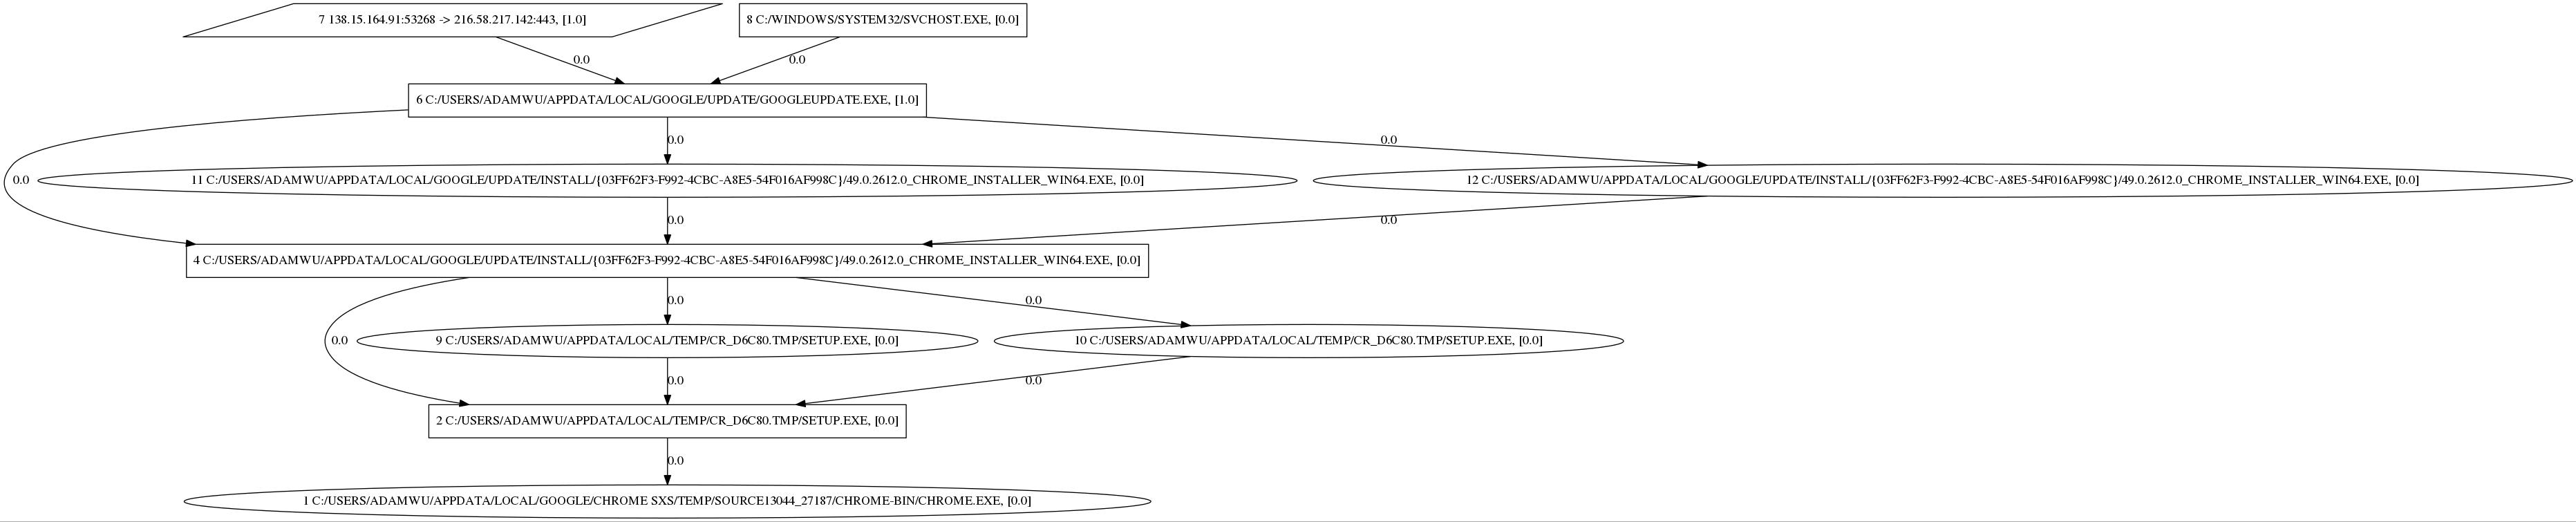
\includegraphics[width=0.5\linewidth,height=5cm]{splitTest.jpg}%
%		\label{fig:b}%
%	}%
%	\caption{The test sample of Graph Split}
%	\label{fig:sampleResult}
%\end{figure*}